%
%  intro.tex
%
%  Created by Drew Conway on 2011-01-26
% 
%
\documentclass[xcolor=dvipsnames, 9pt]{beamer}

\usepackage{amssymb}
\usepackage{amsfonts}
\usepackage{amsmath}
\usepackage{hyperref}
\usepackage{natbib}
\usepackage{color}
\usepackage{pdfsync}
\usepackage{chancery}
\usepackage{movie15}
\usepackage{pgfpages}
\usepackage{fancyvrb}
\usepackage{colortbl}
\usepackage{multirow}

\usepackage{graphicx}
\graphicspath{{../../images/figures/}{../../images/logos/}{../../images/graphs/}/}

\usepackage{beamerthemesplit}
\usetheme{Copenhagen}
\definecolor{title}{RGB}{128,148,182}
\usecolortheme[named=title]{structure} 
\setbeamertemplate{headline}{}
\setbeamertemplate{navigation symbols}{}
\setbeamertemplate{itemize items}[triangle]
\setbeamertemplate{enumerate items}[default]
\setbeamertemplate{footline}[page number]{}
%\setbeameroption{show notes on second screen}


\usepackage{listings}
%\usepackage{listings,arev}
\definecolor{keywords}{RGB}{128,148,182}
\definecolor{comments}{RGB}{60,179,113}
\lstset{numbers=left,
        showstringspaces=false,
        numberstyle=\tiny,
        %frame=leftline,
        numbersep=4.5pt,
  keywordstyle=\color{keywords}\bfseries,
  commentstyle=\color{YellowOrange}\emph
}

\newenvironment{code}{\begin{semiverbatim} \begin{footnotesize}}
{\end{footnotesize}\end{semiverbatim}}

% references
\newcommand{\fref}[1]{Figure~\ref{#1}}
\newcommand{\eref}[1]{Equation~\ref{#1}}
\newcommand{\aref}[1]{Algorithm~\ref{#1}}
\newcommand{\cref}[1]{Chapter~\ref{#1}}
\newcommand{\sref}[1]{Section~\ref{#1}}
\newcommand{\apref}[1]{Appendix~\ref{#1}}

% beamer
\newcommand{\alertb}[1]{\textbf{\alert{#1}}}
\newcommand{\structureb}[1]{\textbf{\structure{#1}}}
\newcommand{\fractext}[2]{{\text{#1} \over \text{#2}}}

% naive bayes (roman for words, class and probabilities)
\newcommand{\class}{\textrm{class}}
\newcommand{\word}{\textrm{word}}
\newcommand{\words}{\textrm{words}}
\newcommand{\Pwsgc}{\Pxgy{\words}{\class}}
\newcommand{\Pwgc}{\Pxgy{\word}{\class}}
\newcommand{\Pcgws}{\Pxgy{\class}{\words}}
\newcommand{\Pc}{\Px{\class}}
\newcommand{\Pws}{\Px{\words}}
\newcommand{\PwsgcT}{\Pxgy{\words}{\class,\T}}
\newcommand{\PcgwsT}{\Pxgy{\class}{\words,\T}}
\newcommand{\PcT}{\Px{\class,\T}}
\newcommand{\PwsT}{\Px{\words,\T}}
\newcommand{\twc}{\theta_{wc}}
\newcommand{\thatwc}{\hat{\theta}_{wc}}
\newcommand{\thatc}{\hat{\theta}_{c}}
\newcommand{\Nwc}{N_{wc}}
\newcommand{\Nc}{N_c}

% widths for figure handling
\newcommand{\fullwidth}{\textwidth}
\newcommand{\halfwidth}{.45\textwidth}
\newcommand{\thirdwidth}{.3\textwidth}
\newcommand{\quarterwidth}{.25\textwidth}
\newcommand{\threequarterwidth}{.75\textwidth}

% general math (exponentials, partial derivatives)
\newcommand{\e}[1]{\operatorname{e}^{#1}}
\newcommand{\R}{\mathbb{R}}
\newcommand{\dfdx}[2]{{d #1 \over d #2}}
\newcommand{\DfDx}[2]{{\partial #1 \over \partial #2}}
\newcommand{\DxDf}[2]{{\partial #2 \over \partial #1}}
\renewcommand{\d}{\mathsf{d}}
\newcommand{\dd}{\partial}
\newcommand{\E}{\mathsf{E}}
\newcommand{\bb}{\mathbf}

% argmax, argmin, vect
%\newcommand{\argmax}[1]{argmax_{#1}}
%\newcommand{\argmax}{\arg\max}
\newcommand{\argmax}[1]{\underset{#1}{\operatorname{argmax}}\,}
\newcommand{\argmin}[1]{\underset{#1}{\operatorname{argmin}}\,}
\newcommand{\vect}[1]{\ensuremath{\vec{#1}}}

% probabilities (joint, conditional, etc.)
\newcommand{\RV}[1]{\uppercase{#1}}
\renewcommand{\SS}[1]{\Omega_{\RV{#1}}}
\newcommand{\PX}[1]{p_{\RV{#1}}\left(\RV{#1}\right)}
\newcommand{\PXeqx}[2]{p_{\RV{#1}}\left(\RV{#1}=#2\right)}
\newcommand{\PXx}[1]{p_{\RV{#1}}\left(#1\right)}
\newcommand{\Px}[1]{p\left(\lowercase{#1}\right)}
\newcommand{\Qx}[1]{q\left(\lowercase{#1}\right)}
\newcommand{\sumSS}[1]{\sum_{\lowercase{#1}\in\SS{#1}}}
\newcommand{\pX}[1]{p_{\RV{#1}}\left(\RV{#1}\right)}
\newcommand{\pXeqx}[2]{p_{\RV{#1}}\left(\RV{#1}=#2\right)}
\newcommand{\pXx}[1]{p_{\RV{#1}}\left(#1\right)}
\newcommand{\px}[1]{p\left(#1\right)}
\newcommand{\intSS}[1]{\int_{\SS{#1}} d\lowercase{#1} \ }
\newcommand{\PXYeqxy}[2]{p_{\RV{#1#2}}\left(\RV{#1}=\lowercase{#1},\RV{#2}=\lowercase{#2}\right)}
\newcommand{\Pxy}[2]{p\left(\lowercase{#1},\lowercase{#2}\right)}
\newcommand{\PXgYeqxgy}[2]{p_{\RV{#1|#2}}\left(\RV{#1}=\lowercase{#1}|\RV{#2}=\lowercase{#2}\right)}
\newcommand{\Pxgy}[2]{p\left(\lowercase{#1}|\lowercase{#2}\right)}
\newcommand{\vx}{\vect{x}}
\newcommand{\veta}{\vect{\eta}}
\newcommand{\vuvx}{\vect{u}(\vx)}

% information theory (entropy, kl divergence)
\newcommand{\SX}[1]{S\left[\RV{#1}\right]}
\newcommand{\Sp}[1]{S\left[p\right]}
\newcommand{\SPx}[1]{S\left[#1\right]}
\newcommand{\xlogx}[1]{#1 \ln #1}
\newcommand{\DKLPQ}[2]{D_{KL}\left[#1||#2\right]}
\newcommand{\xlogxovery}[2]{#1 \ln {#1 \over #2}}
\newcommand{\MIPxy}[1]{I\left[#1\right]}

% probabilities, ML style (D=observed data, Z=latent data, T=params)
\newcommand{\D}{\mathcal{D}}
\newcommand{\Z}{Z}
\newcommand{\T}{\Theta}
\newcommand{\TML}{\T_{ML}}
\newcommand{\K}{K}
\newcommand{\Kstar}{\K^*}
\newcommand{\M}{\mathcal{M}}
\newcommand{\prob}[1]{p(#1)}
\newcommand{\probg}[2]{\prob{#1|#2}}
\newcommand{\probq}[1]{q(#1)}
\newcommand{\probqg}[2]{\probq{#1|#2}}
\newcommand{\pDgT}{\probg{\D}{\T}}
\newcommand{\pDZT}{\prob{\D,\Z,\T}}
\newcommand{\pDZTgK}{\probg{\D,\Z,\T}{\K}}
\newcommand{\pZTgD}{\probg{\Z,\T}{\D}}
\newcommand{\pDgTZ}{\probg{\D}{\T,\Z}}
\newcommand{\pTZ}{\prob{\T,\Z}}
\newcommand{\pD}{\prob{\D}}
\newcommand{\pDgK}{\probg{\D}{\K}}
\newcommand{\pKgD}{\probg{\K}{\D}}
\newcommand{\pK}{\prob{\K}}
\newcommand{\pDgM}{\probg{\D}{\M}}
\newcommand{\pMgD}{\probg{\M}{\D}}
\newcommand{\pM}{\prob{\M}}
\newcommand{\pTK}{\prob{\T,\K}}
\newcommand{\pTKgD}{\probg{\T,\K}{\D}}
\newcommand{\pTgK}{\probg{\T}{\K}}
\newcommand{\pDgTK}{\probg{\D}{\T,\K}}
\newcommand{\pTgD}{\probg{\T}{\D}}
\newcommand{\pTgDK}{\probg{\T}{\D,\K}}
\newcommand{\pDZgT}{\probg{\D,\Z}{\T}}
\newcommand{\pZgDT}{\probg{\Z}{\D,\T}}
\newcommand{\pDZgTK}{\probg{\D,\Z}{\T,\K}}
\newcommand{\pZTgDK}{\probg{\Z,\T}{\D,\K}}

% regression 
\newcommand{\xiyi}{(x_i,y_i)}
\newcommand{\xiyiN}{\{\xiyi\}_{i=1}^N}
\newcommand{\xiN}{\{x_i\}_{i=1}^N}
\newcommand{\yiN}{\{y_i\}_{i=1}^N}
\newcommand{\tkK}{\{\theta_k\}_{k=0}^K}
\newcommand{\ft}[1]{f_{\theta}(#1)}
\newcommand{\ftx}{\ft{x}}
\newcommand{\ftxi}{\ft{x_i}}
\newcommand{\xik}{(x_i)^k}

% gaussians
\newcommand{\sigsq}{\sigma^2}
\newcommand{\twosigsqinv}{{1 \over 2\sigsq}}
\newcommand{\twopisigsq}{2\pi\sigsq}
\newcommand{\twopisigsqinv}{{1 \over \sqrt{\twopisigsq}}}
\newcommand{\Norm}[2]{\mathcal{N}\left(#1|#2\right)}

% clustering
\newcommand{\ziN}{\{z_i\}_{i=1}^N}
\newcommand{\muk}{\mu_k}
\newcommand{\mukp}{\mu_{k'}}
\newcommand{\sigsqk}{\sigma^2_k}
\newcommand{\sigsqkp}{\sigma^2_{k'}}
\newcommand{\pik}{\pi_k}
\newcommand{\musigsqpikK}{\{\muk,\sigsqk,\pik\}_{k=1}^K}
\newcommand{\muzi}{\mu_{z_i}}
\newcommand{\sigsqzi}{\sigsq_{z_i}}
\newcommand{\pxzgT}{\probg{\xiN,\ziN}{\T}}
\newcommand{\pzigT}{\probg{z_i}{\T}}
\newcommand{\pzikgT}{\probg{z_i=k}{\T}}
\newcommand{\pxigT}{\probg{x_i}{\T}}
\newcommand{\pxigziT}{\probg{x_i}{z_i,\T}}
\newcommand{\qZ}{\probq{Z}}
\newcommand{\deltakkp}{\delta_{k,k'}}
\newcommand{\pikp}{\pi_{k'}}
\newcommand{\Qikp}{Q_{ik'}}
\newcommand{\Qipkp}{Q_{i'k'}}

% gaussian mixture models
\newcommand{\sumvz}{\sum_{\vz}}
\newcommand{\pxzgt}{\probg{\vx,\vz}{\vtheta}}
\newcommand{\pxizigt}{\probg{x_i,z_i}{\vtheta}}
\newcommand{\pxigzit}{\probg{x_i}{z_i,\vtheta}}
\newcommand{\pxigzikt}{\probg{x_i}{z_i=k,\vtheta}}
\newcommand{\pzigt}{\probg{z_i}{\vtheta}}
\newcommand{\pzigxit}{\probg{z_i}{x_i,\vtheta}}
\newcommand{\pzikgt}{\probg{z_i=k}{\vtheta}}
\newcommand{\pzikgxit}{\probg{z_i=k}{x_i,\vtheta}}
\newcommand{\normpdf}[3]{{1\over\sqrt{2\pi #3}} \e{-{1\over 2 #3} \left( #1 - #2 \right)^2}}
\newcommand{\pxgt}{\probg{x}{\vtheta}}
\newcommand{\pxigt}{\probg{x_i}{\vtheta}}
\newcommand{\pxizikgt}{\probg{x_i,z_i=k}{\vtheta}}
\newcommand{\deltaiip}{\delta_{i,i'}}
\newcommand{\pxigzikpt}{\probg{x_i}{z_i=k',\vtheta}}

% maximum likelihood EM
\newcommand{\Tinit}{\T^{(0)}}
\newcommand{\Told}{\T^{(t)}}
\newcommand{\Tnew}{\T^{(t+1)}}
\newcommand{\qZold}{q^{(t)}(\Z)}
\newcommand{\qZnew}{q^{(t+1)}(\Z)}
\newcommand{\FqZTold}{\F[\qZ,\Told]}
\newcommand{\FqZoldT}{\F[\qZold,\T]}
\newcommand{\FqZnewT}{\F[\qZnew,\T]}
\newcommand{\FqZoldTold}{\F[\qZold,\Told]}
\newcommand{\FqZnewTnew}{\F[\qZnew,\Tnew]}
\newcommand{\FpZgDTT}{\F[\pZgDT,\T]}

% variational EM
\newcommand{\qZT}{\probq{\Z,\T}}
\newcommand{\qT}{\probq{\T}}
\newcommand{\qZinit}{q^{(0)}(\Z)}
\newcommand{\qTinit}{q^{(0)}(\T)}
\newcommand{\qTold}{q^{(t)}(\T)}
\newcommand{\qTnew}{q^{(t+1)}(\T)}
\newcommand{\FqZoldqTold}{\F[\qZold,\qTold]}
\newcommand{\FqZnewqTnew}{\F[\qZnew,\qTnew]}
\newcommand{\FqZqTold}{\F[\qZ,\qTold]}
\newcommand{\FqZoldqT}{\F[\qZold,\qT]}
\newcommand{\FpZTgDK}{\F[\pZTgDK]}
%\newcommand{\FpZgDTT}{\F\{\pZgDT,\T\}}

% sums, integrals and products
\newcommand{\sumkK}{\sum_{k=1}^K}
\newcommand{\sumkpK}{\sum_{k'=1}^K}
\newcommand{\sumiN}{\sum_{i=1}^N}
\newcommand{\prodiN}{\prod_{i=1}^N}
\newcommand{\intT}{\int \! \! d\T \ }
\newcommand{\sumziN}{\sum_{\ziN}}
\newcommand{\sumZ}{\sum_{\Z}}
\newcommand{\sumzs}{\sum_{z_1=1}^{\K} \cdots \sum_{z_N=1}^{\K}}

% big-Oh for computational time / complexity
\newcommand{\Oh}[1]{\mathcal{O}(#1)}

% image segmentation
\newcommand{\h}[1]{h\left(#1\right)}
\newcommand{\hxiyi}{\h{x_i,y_i}}
\newcommand{\hiN}{\left\{h_i\right\}_{i=1}^N}
\newcommand{\phigziT}{\probg{h_i}{z_i,\T}}
\newcommand{\Normhi}{\Norm{h_i}{\muzi,\sigsqzi}}
\newcommand{\Normhik}{\Norm{h_i}{\muk,\sigsqk}}
\newcommand{\pzigTone}{\probg{z_i=1}{\T}}
\newcommand{\pzigTtwo}{\probg{z_i=2}{\T}}
\newcommand{\Normhione}{\Norm{h_i}{\mu_1,\sigsq_1}}
\newcommand{\Normhitwo}{\Norm{h_i}{\mu_2,\sigsq_2}}
\newcommand{\mukold}{\muk^{(t)}}
\newcommand{\muknew}{\muk^{(t+1)}}
\newcommand{\sigsqkold}{\sigma^{2,(t)}_k}
\newcommand{\sigsqknew}{\sigma^{2,(t+1)}_k}
\newcommand{\pikold}{\pik^{(t)}}
\newcommand{\piknew}{\pik^{(t+1)}}
\newcommand{\Normhikold}{\Norm{h_i}{\mukold,\sigsqkold}}
\newcommand{\Normhikpold}{\Norm{h_i}{\mu_{k'}^{(t)},\sigma_{k'}^{2,(t)}}}
\newcommand{\Qik}{Q_{ik}}
\newcommand{\Qikold}{Q_{ik}^{(t)}}
\newcommand{\Qiknew}{Q_{ik}^{(t+1)}}

% random aliases from vbmod prl
\newcommand{\Jensen}{Gibbs}
\newcommand{\myspace}{\hspace{.8 cm}}
\newcommand{\mA}{\mathbf{A}}
\newcommand{\Pij}{P_{ij}}
\newcommand{\Aij}{A_{ij}}
\newcommand{\Aji}{A_{ji}}
\newcommand{\thetap}{\theta_+}
\newcommand{\thetam}{\theta_-}
\newcommand{\thetapm}{\theta_{\pm}}
\newcommand{\vz}{\vect{z}}
\newcommand{\vtheta}{\vect{\theta}}
\newcommand{\vpi}{\vect{\pi}}
%\newcommand{\pik}{\pi_k}
\newcommand{\prodk}{\prod_{k=1}^K}
\newcommand{\prodn}{\prod_{i=1}^N}
\newcommand{\prodi}{\prod_{i=1}^N}
\newcommand{\prodij}{\prod_{i>j}}
\newcommand{\sumij}{\sum_{i>j}}
\newcommand{\sumk}{\sum_{k=1}^K}
\newcommand{\sumz}{\sum_{\vz}}
\newcommand{\intpi}{\int \!\! d\vpi}
\newcommand{\inttheta}{\int \!\! d\vtheta}
\newcommand{\intthetap}{\int \!\! d\thetap}
\newcommand{\intthetam}{\int \!\! d\thetam}
\newcommand{\ptheta}{p(\vtheta)}
\newcommand{\pthetap}{p(\thetap)}
\newcommand{\pthetam}{p(\thetam)}
\newcommand{\ppi}{p(\vpi)}
\newcommand{\ptp}{p(\thetap)}
\newcommand{\ptm}{p(\thetam)}
\newcommand{\ppit}{p(\vpi,\vtheta)}
\newcommand{\pzigpi}{p(z_i|\vpi)}
\newcommand{\pz}{p(\vz)}
\newcommand{\pzik}{p(z_i=k|\vpi)}
\newcommand{\pzimu}{p(z_i=\mu|\vpi)}
\newcommand{\pAijgzizj}{p(\Aij|z_i,z_j,\vtheta)}
\newcommand{\npp}{n_{++}}
\newcommand{\npm}{n_{+-}}
\newcommand{\nmp}{n_{-+}}
\newcommand{\nmm}{n_{--}}
\newcommand{\ntpp}{\tilde{n}_{++}}
\newcommand{\ntpm}{\tilde{n}_{+-}}
\newcommand{\ntmp}{\tilde{n}_{-+}}
\newcommand{\ntmm}{\tilde{n}_{--}}
\newcommand{\nk}{n_k}
\newcommand{\deltazizj}{\delta_{z_i,z_j}}
\newcommand{\distAijp}{\thetap^{\Aij}(1-\thetap)^{1-\Aij} \deltazizj}
\newcommand{\distAijm}{\thetam^{\Aij}(1-\thetam)^{1-\Aij} (1-\deltazizj)}
\newcommand{\sumi}{\sum_{i=1}^N}
\newcommand{\deltazik}{\delta_{z_i,k}}
\newcommand{\deltazia}{\delta_{z_i,\alpha}}
\newcommand{\vzrg}{\vect{z}_{rg}}
\newcommand{\sumzrg}{\sum_{\vz_{rg}}}
\newcommand{\knz}{K_{nz}}
\newcommand{\kpknz}{{}_KP_{\knz}}
\newcommand{\pzrg}{p(\vzrg)}
\newcommand{\pAzpit}{p(\mA,\vz,\vpi,\vtheta)}
\newcommand{\qztpi}{q(\vz,\vtheta,\vpi)}
\newcommand{\Qz}{q_{\vz}(\vz)}
\newcommand{\qz}[1]{q_{z_{#1}}(z_{#1})}
\newcommand{\Qt}{q_{\vtheta}(\vtheta)}
\newcommand{\Qtp}{q_+(\thetap)}
\newcommand{\Qtm}{q_-(\thetam)}
\newcommand{\ap}{\alpha_+}
\newcommand{\am}{\alpha_-}
\newcommand{\bp}{\beta_+}
\newcommand{\bm}{\beta_-}
\newcommand{\apt}{\tilde{\alpha}_+}
\newcommand{\amt}{\tilde{\alpha}_-}
\newcommand{\bpt}{\tilde{\beta}_+}
\newcommand{\bmt}{\tilde{\beta}_-}
\newcommand{\Qtpab}{Q_+(\thetap;\ap,\bp)}
\newcommand{\Qtmab}{Q_-(\thetam;\am,\bm)}
\newcommand{\Qpi}{Q_{\vpi}(\vpi)}
\newcommand{\expval}[1]{\left\langle #1 \right\rangle}
%\newcommand{\E}[2]{\mathbb{E}_{#1}\left[ #2 \right]}
\newcommand{\FQA}{F[Q;\mA]}
\newcommand{\na}{\nmu}
\newcommand{\pia}{\pimu}
\newcommand{\suma}{\sum_{\mu=1}^K}
\newcommand{\sumzi}{\sum_{z_i}}
\newcommand{\sumzj}{\sum_{z_j}}
\newcommand{\mQ}{\mathbf{Q}}
\newcommand{\Qia}{Q_{i\mu}}
\newcommand{\Qja}{Q_{j\mu}}
\newcommand{\Qlb}{Q_{l\nu}}
\newcommand{\Qjb}{Q_{j\nu}}
\newcommand{\Qimu}{Q_{i\mu}}
\newcommand{\Qjmu}{Q_{j\mu}}
\newcommand{\Qinu}{Q_{i\nu}}
\newcommand{\Qjnu}{Q_{j\nu}}
\newcommand{\Alj}{A_{lj}}
%\newcommand{\D}[2]{\frac{\partial #2}{\partial #1}}
\newcommand{\sumj}{\sum_{j=1}^N}
\newcommand{\mAQ}{\mA\mQ}
\newcommand{\mAQlb}{(\mA\mQ)_{l\nu}}
\newcommand{\enpp}{\expval{\npp}}
\newcommand{\enpm}{\expval{\npm}}
\newcommand{\enmp}{\expval{\nmp}}
\newcommand{\enmm}{\expval{\nmm}}
\newcommand{\enmu}{\expval{\nmu}}
\newcommand{\elntp}{\expval{\ln\thetap}}
\newcommand{\elnmtp}{\expval{\ln(1-\thetap)}}
\newcommand{\elntm}{\expval{\ln\thetam}}
\newcommand{\elnmtm}{\expval{\ln(1-\thetam)}}
\newcommand{\va}{\vect{\alpha}}
\newcommand{\prodmu}{\prod_{\mu=1}^K}
\newcommand{\prodmuneqnu}{\prod_{\mu\neq\nu}}
\newcommand{\summu}{\sum_{\mu=1}^K}
\newcommand{\pizi}{\pi_{z_i}}
\newcommand{\pimu}{\pi_{\mu}}
\newcommand{\pinu}{\pi_{\nu}}
\newcommand{\nmu}{n_{\mu}}
\newcommand{\amu}{\alpha_{\mu}}
\newcommand{\anu}{\alpha_{\nu}}
\newcommand{\amut}{\tilde{\amu}}
\newcommand{\elnnmu}{\expval{\nmu}}
\newcommand{\elnpimu}{\expval{\ln\pimu}}
\newcommand{\elnpinu}{\expval{\ln\pinu}}
\newcommand{\Jq}{J(q)}
\newcommand{\Js}{\tilde{J}(s)}
\newcommand{\lap}[1]{\mathcal{L}\left\{ #1 \right\}}
\newcommand{\invlap}[1]{\mathcal{L}^{-1}\left\{ #1 \right\}}
\newcommand{\pAgzpit}{p(\mA|\vz,\vpi,\vtheta)}
\newcommand{\pAgt}{p(\mA|\theta)}
\newcommand{\pAgzt}{p(\mA|\vz,\vtheta)}
\newcommand{\pzgpi}{p(\vz|\vpi)}
\newcommand{\pAzgpit}{p(\mA,\vz|\vpi,\vtheta)}
\newcommand{\EAzgpit}{E(\mA,\vz;\vpi,\vtheta)}
\newcommand{\pA}{p(\mA)}
\newcommand{\pAz}{p(\mA,\vz)}
\newcommand{\pAgz}{p(\mA|\vz)}
\newcommand{\eJ}{\expval{J_L}}
\newcommand{\eJp}{\expval{J_G}}
\newcommand{\SQz}{S_{\Qz}}
\newcommand{\SQp}{S_{\Qtp}}
\newcommand{\SQm}{S_{\Qtm}}
\newcommand{\SQpi}{S_{\Qpi}}
\newcommand{\elnptp}{\expval{\ln\ptp}}
\newcommand{\elnptm}{\expval{\ln\ptm}}
\newcommand{\elnppi}{\expval{\ln\ppi}}
%\newcommand{\Z}{\mathcal{Z}}
\newcommand{\Zp}{\Zda_+}
\newcommand{\Zm}{\Zda_-}
\newcommand{\Zpi}{\Zda_{\vpi}}
\newcommand{\Zpt}{\tilde{\Zda}_+}
\newcommand{\Zmt}{\tilde{\Zda}_-}
\newcommand{\Zpit}{\tilde{\Zda}_{\vpi}}
%\newcommand{\data}{\mathcal{D}}
%\newcommand{\param}{\Theta}
%\newcommand{\hidvar}{Z}
%\newcommand{\pD}{p(\data)}
\newcommand{\pT}{p(\T)}
\newcommand{\prx}{p(x)}
\newcommand{\psrx}{p^*(x)}
\newcommand{\psrxr}{p^*(\xr)}
\newcommand{\qrx}{q(x)}
\newcommand{\qsrx}{q^*(x)}
\newcommand{\qsrxr}{q^*(\xr)}
\newcommand{\fx}{\phi(x)}
\newcommand{\xr}{x^{(r)}}
\newcommand{\fxr}{\phi(\xr)}
\newcommand{\intx}{\int \! \! dx}
\newcommand{\sumR}{\sum_{r=1}^R}
\newcommand{\Phihat}{\widehat{\Phi}}
\newcommand{\xt}{x^{(t)}}
\newcommand{\xtpo}{x^{(t+1)}}
\newcommand{\qrxpt}{q(x';\xt)}
\newcommand{\qrxtp}{q(\xt;x')}
\newcommand{\psrxt}{p^*(\xt)}
\newcommand{\psrxp}{p^*(x')}
%\newcommand{\qZT}{q(\hidvar,\param)}
%\newcommand{\pDZT}{p(\D,\Z,\T)}
%\newcommand{\pZTgD}{p(\Z,\T | \D)}
\newcommand{\sumZintT}{\sum_{\Z} \int d\T \ }
\newcommand{\DKL}{D_{KL}}
\newcommand{\DKLqZTpZTgD}{\DKL\left(\qZT||\pZTgD\right)}
\newcommand{\spin}{\vect{\sigma}}
\newcommand{\sumS}{\sum_{\spin} \ }
\newcommand{\sumSintT}{\sum_{\spin} \int d\T \ }
\newcommand{\hamiltonian}{\mathcal{H}}
\newcommand{\Htest}{\hamiltonian^0}
\newcommand{\Ztest}{\Z^0}
\newcommand{\Zda}{\mathcal{Z}}
\newcommand{\Zdatest}{\mathcal{Z}^0}
\newcommand{\Hspin}{\hamiltonian_{\spin|\T}}
\newcommand{\expvaltest}[1]{\expval{#1}^0}
\newcommand{\Hparam}{\hamiltonian_{\T}}
\newcommand{\Zparam}{\Z_{\T}}
\newcommand{\Hparamtest}{\Hparam^0}
\newcommand{\Hspintest}{\Hspin^0}
\newcommand{\deltasisj}{\delta_{z_i,z_j}}
\newcommand{\deltasimu}{\delta_{z_i,\mu}}
\newcommand{\hmu}{h_{\mu}}
\newcommand{\vh}{\vect{h}}
% change back for c,d notation
%\renewcommand{\npp}{c_+}
%\renewcommand{\npm}{c_-}
%\renewcommand{\nmp}{d_+}
%\renewcommand{\nmm}{d_-}
%\renewcommand{\thetap}{\theta_c}
%\renewcommand{\thetam}{\theta_d}
%\renewcommand{\ap}{\tilde{c}_+}
%\newcommand{\apm}{\tilde{c}_{\pm}}
\newcommand{\apm}{\alpha_{\pm}}
%\renewcommand{\apt}{\tilde{c}_{+_0}}
%\renewcommand{\bp}{\tilde{c}_-}
%\newcommand{\bpm}{\tilde{d}_\pm}
\newcommand{\bpm}{\beta_{\pm}}
%\renewcommand{\bpt}{\tilde{c}_{-_0}}
%\renewcommand{\am}{\tilde{d}_+}
%\renewcommand{\amt}{\tilde{d}_{+_0}}
%\renewcommand{\bm}{\tilde{d}_-}
%\renewcommand{\bmt}{\tilde{d}_{-_0}}
%\renewcommand{\va}{\tilde{\vect{n}}}
%\renewcommand{\vn}{\vect{n}}
\newcommand{\vn}{\vect{n}}
%\renewcommand{\amu}{\tilde{n}_{\mu}}
%\renewcommand{\amut}{\tilde{n}_{\mu_0}}
\newcommand{\si}{z_i}
\newcommand{\sj}{z_j}
\newcommand{\vs}{\vect{z}}
\newcommand{\sums}{\sum_{\vs}}
\newcommand{\sumn}{\sum_{<i,j>}}
\newcommand{\sumnn}{\sum_{<i,j>'}}
%\newcommand{\deltasisj}{\delta_{\si,\sj}}
%\newcommand{\deltasimu}{\delta_{\si,\mu}}
\newcommand{\sumlocal}{\sumij \Aij \deltazizj}
\newcommand{\sumglobal}{\sumij \deltazizj}
\newcommand{\sumglobalocc}{{1\over2}\summu \nmu(\nmu-1)}
\newcommand{\sumnpp}{\sumlocal}
\newcommand{\sumnpm}{\sumij (1-\Aij) \deltazizj}
\newcommand{\sumnmp}{\sumij \Aij (1-\deltazizj)}
\newcommand{\sumnmm}{\sumij (1-\Aij) (1-\deltazizj)}
%\newcommand{\sumnpp}{\sumn \deltasisj}
%\newcommand{\sumnpm}{\sumnn \deltasisj}
%\newcommand{\sumnmp}{\sumn (1-\deltasisj)}
%\newcommand{\sumnmm}{\sumnn (1-\deltasisj)}
\newcommand{\sumnmu}{\summu \deltazimu}
\newcommand{\Nedges}{M}
\newcommand{\Nedgessq}{C}
\renewcommand{\vtheta}{\vect{\theta}}
%\renewcommand{\inttheta}{\int \!\! d\thetap \int \!\! d\thetam}
\newcommand{\pAspit}{p(\mA,\vs,\vpi,\vtheta|K)}
\newcommand{\pAgspit}{p(\mA|\vs,\vtheta)}
\newcommand{\pAsgpitK}{p(\mA,\vs|\vpi,\vtheta,K)}
\newcommand{\pAsgpit}{p(\mA,\vs|\vpi,\vtheta)}
\newcommand{\psgpi}{p(\vs|\vpi)}
\newcommand{\ppitgA}{p(\vpi,\vtheta|\mA)}
\newcommand{\psgA}{p(\vs|\mA)}
\newcommand{\pAgK}{p(\mA|K)}
\newcommand{\qspit}{q(\vs,\vpi,\vtheta)}
\renewcommand{\FQA}{F[\qspit]}
\newcommand{\qs}{q_{\vs}(\vs)}
\newcommand{\qpi}{q_{\vpi}(\vpi)}
\newcommand{\qt}{q_{\vtheta}(\vtheta)}
\newcommand{\qc}{q_+(\thetap)}
\newcommand{\qd}{q_-(\thetam)}
\newcommand{\pc}{p_+(\thetap)}
\newcommand{\pd}{p_-(\thetam)}
\newcommand{\ZQ}{\Z_Q}
\renewcommand{\Zp}{\Zda_+}
\renewcommand{\Zm}{\Zda_-}
\renewcommand{\Zpt}{\tilde{\Zda}_+}
\renewcommand{\Zmt}{\tilde{\Zda}_-}
\renewcommand{\Hspin}{\hamiltonian}
\renewcommand{\Hparam}{\hamiltonian_{\vtheta,\vpi}}
%\renewcommand{\expvaltest}[1]{\expval{#1}_{\Htest}}
% added 2008.07.13
\newcommand{\Jij}{J_{ij}}
\newcommand{\eJij}{\expval{J_{ij}}}
\newcommand{\eJik}{\expval{J_{ik}}}
\newcommand{\lnpimu}{\ln \pimu}
\newcommand{\deltazimu}{\delta_{z_i,\mu}}
\newcommand{\deltaij}{\delta_{ij}}
\newcommand{\deltaik}{\delta_{ik}}
\newcommand{\deltazizk}{\delta_{z_i,z_k}}
\newcommand{\znoti}{\vect{z}_{-i}}
\newcommand{\sumjneql}{\sum_{j \neq l}}

% beta and dirichlet distributions
\newcommand{\betafcn}[2]{B(#1,#2)}
\newcommand{\betafcnv}[1]{B(#1)}
\newcommand{\betapdf}[3]{{#1^{#2-1}(1-#1)^{#3-1} \over \betafcn{#2}{#3}}}
\newcommand{\dirfcn}[1]{\Gamma(#1)}
\newcommand{\dirpdf}[2]{{1 \over \betafcnv{\vect{#2}}} \prod_{\mu=1}^{K} #1_{\mu}^{#2_{\mu}-1}}



\title{Visualization Basics}
\author{Joseph Adler, Drew Conway, Jake Hofman, Hilary Mason}
\date{February 1, 2011}

\begin{document} 
    
\begin{frame}[plain]
  \titlepage 

  \tiny
  \href{http://creativecommons.org/licenses/by-sa/3.0/us/}{\includegraphics[width=1cm]{ccbysa}}

  Creative Commons Attribution-Share Alike 3.0
\end{frame}

\section{Data Visualization Introduction} % (fold)
\label{sec:visualization}

\subsection{What data visualization should do} % (fold)
\label{sub:what_data_visualization_should_do}

{
\setbeamercolor{background canvas}{bg=}
\usebackgroundtemplate{\includegraphics[width=\paperwidth,
height=\paperheight]{Afgan-orig-med.jpg}}
\begin{frame}[fragile]
    \frametitle{}
    \vspace{4cm}
    \begin{center}
        \begin{minipage}{5cm}
        \uncover<2->{\begin{varblock}[6cm]{What data visualization should do?}
            \begin{enumerate}
                \uncover<3->{\item Make complex ideas \textbf{simple}}
                \uncover<4->{\item Extract \textbf{small} info from big data}
                \uncover<5->{\item Present \textbf{truth}, not deceive}
            \end{enumerate}
        \end{varblock}}
    \end{minipage}
    \end{center}
\end{frame}
}

\begin{frame}[fragile]
    \frametitle{Make complex ideas \textbf{simple}}
    \begin{center}
        \only<1>{\includegraphics[height=8cm,clip,trim=0cm 5cm 0cm 5cm]{full_ibes_weighted_mc}}
        \only<2>{\includegraphics[height=8cm,clip,trim=0cm 5cm 0cm 5cm]{full_ibes_weighted_mc_2c_reduce.pdf}}
    \end{center}
\end{frame}

\begin{frame}[fragile]
    \frametitle{Good example of complexity reduction}
    \begin{center}
        \includegraphics[width=11cm]{facebook_map_reduce.png}
    \end{center}
\end{frame}


\begin{frame}[fragile]
    \frametitle{Extract \textbf{small} info from big data}
    \begin{center}
        \only<1>{\includegraphics[width=11cm]{events_by_year_map.png}}
        \only<2>{\includegraphics[width=10cm]{ied_by_year.pdf}}
    \end{center}
\end{frame}

\begin{frame}[fragile]
    \frametitle{Present \textbf{truth}, do not deceive}
    \begin{center}
        \only<1>{\includegraphics[height=8cm,width=10cm]{poli_sci1.png}}
        \only<2>{\includegraphics[height=8cm,width=10cm]{poli_sci2.png}}
    \end{center}
\end{frame}

% subsection what_data_visualization_should_do (end)

\subsection{Data visualization tools} % (fold)
\label{sub:data_visualization_tools}

\begin{frame}[fragile]
    \frametitle{Commercial data visualization tools}
    Data visualization is very popular...
    \begin{center}
        \includegraphics[width=10cm]{google_data_viz_count.png}
        \uncover<2->{\begin{block}{Strata $\heartsuit$'s visualization!}
\tiny{\begin{code}
\$ wget -O strata.htm http://strataconf.com/strata2011/public/schedule/full

\$ tr -cs `A-Za-z' `$\backslash$n' < strata.html | grep -c ``visual''

\alert{24}
\end{code}}
        \end{block}}
    \end{center}
    \uncover<3->{\begin{columns}[c]
        \column{.33\textwidth}
        \includegraphics[width=3cm]{juice_white_small.jpg} \\ \vspace{4mm}
        \includegraphics[width=3cm]{tableau_logo.png} \\ \vspace{4mm}
        \includegraphics[width=3cm]{periscopic.png}
        \column{.33\textwidth}
        \includegraphics[width=3cm]{gooddata.png} \\ \vspace{4mm}
        \includegraphics[width=3cm]{google.png} \\ \vspace{4mm}
        \includegraphics[width=3cm]{digital_reasoning.png}
        \column{.33\textwidth}
        \includegraphics[width=3cm]{readwriteweb-logo.png} \\ \vspace{4mm}
        \includegraphics[width=3cm]{200px-The_New_York_Times_Company_logo.png} \\ \vspace{4mm}
        \includegraphics[width=3cm]{the-guardian-logo.jpg}
    \end{columns}}
\end{frame}

\begin{frame}[fragile]
    \frametitle{Open-source visualization tools}
    For this tutorial we will not be using any commercial tools
    \begin{itemize}
        \item Instead utilizing \textbf{only open-source tools}
    \end{itemize}
    \uncover<2->{There are many tools at our disposal
    \begin{itemize}
        \item Here we will use \textbf{two premier scientific computing environments}
    \end{itemize}}
    \vspace{1cm}
    \uncover<2->{\begin{columns}
        \column{0.5\textwidth}
        \begin{center}
            \includegraphics[width=6cm]{python-logo-master-v3-TM.png}
        \end{center}
        \column{0.5\textwidth}
        \begin{center}
            \includegraphics[height=3cm]{200px-Rlogo.png}
        \end{center}
    \end{columns}}
\end{frame}

\begin{frame}[fragile]
    \frametitle{Python's scientific computing holy trinity}
    \begin{right}
        \uncover<9->{\hfill \textbf{\alert{$\searrow$}\hspace{2cm}\alert{$\swarrow$}}}
    \end{right}
    \begin{columns}
        \column{.33\textwidth}
        \begin{center}
            \href{http://www.scipy.org}{\includegraphics[width=3cm]{Scipylogo.png}}
        \end{center}
        \uncover<2->{Python's primary library for \textbf{mathematical and statistical} computing. Containing sub-libs for
        \begin{itemize}
            \item Numeric optimization
            \item Clustering
            \item Linear algebra
            \item ..and many others
        \end{itemize}}
        \uncover<3->{The primary data type in \texttt{SciPy} is an array
        \begin{itemize}
            \item Data manipulation is similar to that of MATLAB
        \end{itemize}}
        \vspace{3mm}
        \column{.33\textwidth}
        \begin{center}
            \href{http://numpy.scipy.org/}{\includegraphics[clip,trim=0mm 2mm 0mm 2mm,width=2.5cm]{NumPy_logo.png}}
        \end{center}
        \uncover<4->{\texttt{NumPy} is an extension of the \texttt{SciPy} data type to include \textbf{multidimensional arrays and matrices}
        \begin{itemize}
            \item Provides many functions for working on arrays and matrices
            \item Very useful for representing relational data
        \end{itemize}}
        \uncover<5->{Both \texttt{SciPy} and \texttt{NumPy} rely on the C library \texttt{LAPACK} for very fast implementation}
        \column{.33\textwidth}
        \begin{center}
            \href{http://matplotlib.sourceforge.net/}{\includegraphics[width=3cm]{500px-Matplotlib_logo.png}}
        \end{center}
        \uncover<6->{\texttt{matplotlib} is \textbf{primary plotting library in Python}
        \begin{itemize}
            \item Supports 2- and 3-D plotting
            \item API allows embedding in apps
        \end{itemize}}
        \uncover<7->{\includegraphics[width=2cm]{500px-Temp-sunspot-co2.png}
        \includegraphics[width=2cm]{500px-Rosenbrock_function.png}}\\
        \uncover<8->{All graphics are highly customizable and professional publication ready}
    \end{columns}
    \vspace{1mm}
\end{frame}

\begin{frame}[fragile]
    \frametitle{Data visualization in in R}
    \uncover<10->{\hfill \textbf{\alert{$\searrow$}\hspace{1cm}\alert{$\swarrow$}\hspace{1.55cm}}}
    \begin{columns}
        \column{0.33\textwidth}
            \Large{\underline{The \texttt{R} Language}} \\ \vspace{2mm}
            \uncover<2->{\footnotesize{``freely available language and environment for statistical computing and graphics...''}} \\ \vspace{2mm}
            \normalsize
            \uncover<3->{CRAN
            \begin{itemize}
                \item Massive library of specialized packages
                \item 2,775 available
            \end{itemize}}
           \uncover<4->{R Task Views
            \begin{itemize}
                \item 28 development areas
                \item Bayesian, ML, NLP, \textbf{Graphics}
            \end{itemize}}
            \uncover<5->{Two popular visualization packages
            \begin{itemize}
                \item \texttt{lattice}
                \item \texttt{ggplot2}
            \end{itemize}}
        \column{0.33\textwidth}
            \Large{\texttt{\underline{lattice}}} \\ \vspace{2mm}
            \normalsize
            \uncover<6->{Developed by Deepayan Sarkar \\ 
            \includegraphics[height=2.5cm]{Deepayan-Sarkar.png}
            \includegraphics[height=2.5cm]{cleveland.png} \\
            \uncover<7->{\begin{itemize}}
                \item Implementation of Trellis graphics
            \end{itemize}
            \includegraphics[height=2.2cm]{midday_weather_profiles.png}
            \includegraphics[height=2.2cm]{fig09.png}}
        \column{0.33\textwidth}
            \Large{\texttt{\underline{ggplot2}}} \\ \vspace{2mm}
            \normalsize
            \uncover<8->{Developed by Hadley Wickham \\
            \includegraphics[height=2.5cm]{wickham.jpg}
            \includegraphics[height=2.5cm,clip,trim=2mm 0mm 2mm 0mm]{wilkinson.jpg} \\}
            \uncover<9->{\begin{itemize}
                \item Visualizations are ``grammatical layers''
            \end{itemize}
           \includegraphics[width=3cm]{ggplot2_layers.png}\\ \hfill\tiny{Image source: Harlan Harris}}
    \end{columns}
\end{frame}

% subsection data_visualization_tools (end)

\subsection{My first visualization} % (fold)
\label{sub:my_first_visualization}

\begin{frame}[fragile]
    \frametitle{Creating a simple visualization}
    As an introduction to each environment we will make the same plot in both \texttt{matplotlib} and \texttt{ggplot2} \\ 
    \vspace{2mm}
    \uncover<2->{To begin, we'll generate canonical data and visualize it
    \begin{itemize}
        \item Histogram of 10,000 randomly generated numbers from a \textbf{standard Normal distribution}
        \item $\mu = 0$, $\sigma = 1$
        \item Then, overlay Normal density function to observe ``fit''\footnote{Image source: \url{http://mathworld.wolfram.com/NormalDistribution.html}}
    \end{itemize}}
    \uncover<3->{\begin{center}
        \includegraphics[width=5cm]{BinomialGaussian_1000.png}
    \end{center}}
    \uncover<4->{We'll start by working in Python with \texttt{matplotlib}...}
\end{frame}

\begin{frame}[fragile]
    \frametitle{My first \texttt{matplotlib} visualization: 1/3}
    Out first steps are to load the libraries and generate data
    \begin{block}{\texttt{matplotlib} and the normal distribution}
        \begin{lstlisting}[language=Python]
>>> import matplotlib.pylab as plt
>>> from scipy.stats import norm
        \end{lstlisting}
    \end{block}
    \begin{block}{Generate 10,000 random draws from a normal}
        \begin{lstlisting}[language=Python]
>>> random_normal = norm.rvs(0,1,size=10000)
        \end{lstlisting}
    \end{block}
    \begin{block}{Create a \texttt{figure} to draw to}
        \begin{lstlisting}[language=Python]
>>> fig=plt.figure(figsize = (8,6))
        \end{lstlisting}
    \end{block}
\end{frame}

\begin{frame}[fragile]
    \frametitle{My first \texttt{matplotlib} visualization: 2/3}
    Next, we draw the draw to the \texttt{figure}
    \begin{block}{Add the histogram and Normal PDF}
        \begin{lstlisting}[language=Python]
>>> n, bins, pataches = 
    plt.hist(random_numbers,normed=True,bins=25,
    alpha=0.75)  
>>> y = norm.pdf(bins)
>>> plt.plot(bins,y,"r-")
        \end{lstlisting}
    \end{block}
    \begin{block}{Add plot labels, and save}
        \begin{lstlisting}[language=Python]
>>> plt.xlabel("Random numbers")
>>> plt.ylabel("Density")
>>> plt.title("My first matplotlib visualization!")
>>> plt.savefig("matplotlib_first.png")
        \end{lstlisting}
    \end{block}
\end{frame}

\begin{frame}[fragile]
    \frametitle{My first \texttt{matplotlib} visualization: 3/3}
    Now, bask in the glory of your data visualization!
    \begin{center}
        \includegraphics[width=10cm]{matplotlib_first.png}
    \end{center}
\end{frame}

\begin{frame}[fragile]
    \frametitle{My first \texttt{ggplot2} visualization 1/4}
    Again, first load library and create data
    \begin{block}{Load the \texttt{ggplot2} package}
        \begin{lstlisting}[language=R]
> library(ggplot2)
        \end{lstlisting}
    \end{block}
    \begin{block}{Create our first \texttt{data.frame}}
        \begin{lstlisting}[language=R]
> random.numbers<-rnorm(10000,0,1)
> norm.dframe<-as.data.frame(list(Norm=random.numbers))
        \end{lstlisting}
    \end{block}
    \begin{block}{Create base \texttt{ggplot2} layer}
        \begin{lstlisting}[language=R]
> norm.plt<-ggplot(norm.dframe,aes(Norm)) + 
    geom_histogram(aes(y = ..density.., fill="blue", 
    colour="black",alpha=0.75))
        \end{lstlisting}
    \end{block}
\end{frame}

\begin{frame}[fragile]
    \frametitle{My first \texttt{ggplot2} visualization 2/4}
    Next, we build up layers from the base
    \begin{block}{Add Normal PDF}
        \begin{lstlisting}[language=R]
> norm.plt<-norm.plt+stat_function(fun = dnorm, 
        colour = "red")
        \end{lstlisting}
    \end{block} 
    \begin{block}{Deal with colors and legends}
        \begin{lstlisting}[language=R]
> norm.plt<-norm.plt+scale_colour_manual(values = 
        c("black"="black","red"="red"), legend = FALSE)
> norm.plt<-norm.plt+scale_fill_manual(values = 
    c("blue"="blue"), legend = FALSE) 
> norm.plt<-norm.plt+scale_alpha(legend = FALSE)+
        \end{lstlisting}
    \end{block}
\end{frame}

\begin{frame}[fragile]
    \frametitle{My first \texttt{ggplot2} visualization 3/4}
    Finally, add add labels and save
    \begin{block}{This time, we'll make a PDF}
        \begin{lstlisting}[language=R]
> norm.plt<-norm.plt+xlab("Random numbers")
> norm.plt<-norm.plt+ylab("Density")
> norm.plt<-norm.plt+opts(title=
        "My first ggplot2 visualization!")
> ggsave(plot = norm.plt, filename = 
    "ggplot2_first.pdf", height = 6, 
    width = 8)
        \end{lstlisting}
    \end{block}
\end{frame}

\begin{frame}[fragile]
    \frametitle{My first \texttt{ggplot2} visualization 4/4}
    Who's the baddest data visualizer?! You are!
    \begin{center}
        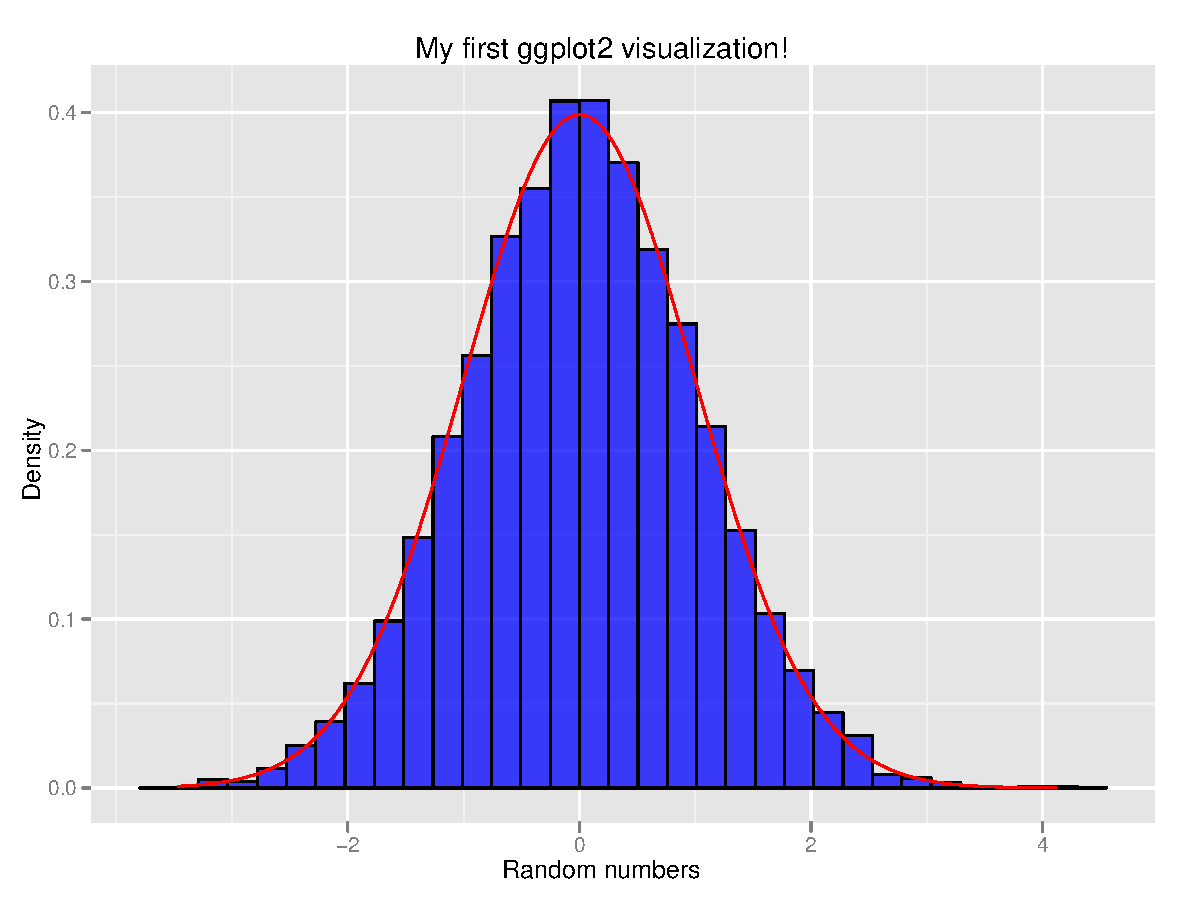
\includegraphics[width=10cm]{ggplot2_first.pdf}
    \end{center}
\end{frame}

% subsection my_first_visualization (end)

% section visualization (end)


\end{document}
